% !TeX root = main.tex
\chapter{Background}\label{chp:background}

Audio is an electronic representation of sound which stores pressure waves as an electrical signal.
Sound is by its very nature time-variant, which makes it both fascinating and challenging.
This temporal property makes it impossible to `freeze' sound, or to experience it in an instant. Listening is a
time-consuming activity, because sound must be consumed over time.

%There have been many attempts to create tools that
%compress the time needed to listen, which are detailed in Section~\ref{sec:background-auditory}.
%These tools still require the user to invest time in the task.

% Sound is linear - has a beginning and an end, constrained by the arrow of time
% Cannot be searched or skimmed
% Sound is one-dimensional
% We never stop listening
% Huge range of frequencies and pressure levels

This also poses a challenge when designed interfaces for interacting with audio content. Dealing with large amounts of
audio in a reasonable time requires the use of tools that can shorten the time needed to complete tasks such as
navigation.

In this chapter, we consider the various approaches that have been used to help users navigate audio content.
A number of approaches have been excluded as they specifically target music content (e.g. chromagrams and music
transcripts).

In section \ref{sec:visualization} we introduce the foundations of audio visualisation and discuss the two most common
visualisation techniques. In section \ref{sec:semantic}, we show how these visualisations can be improved by combining
them with semantic audio analysis techniques. Finally in section \ref{sec:auditory}, we look at non-visual interfaces
to audio, including auditory and haptic techniques.

\section{Audio visualization}\label{sec:visualization}

\citet{Arons1997} found that most humans cannot comprehend speech which it is played faster than twice real-time. This
means that there is a limit on the improvement that can be gained with using continuous audio playback.

Vision is very different medium that varies not only over time, but over space. When you remove the element of time,
you are left with an image that can be experienced instantanously, searched and skimmed.
Human vision can be used to process complex scenes at a glance
%Anderson 2009; Belopolsky et al. 2008; Goldstein 2010
For this reason, visualisation is a good way to interact with time-variant information.
\citet{Aigner2011} contains a collection of examples of how this can be done.

Visual systems can be used to complement audio interfaces, as they are able to address the key challenges of sound.

In modern society, screens for displaying visual content are widely available.

To be able to represent audio visually, we must map auditory properties to visual properties. We could select these 
to have a general mapping, which attempts to cover all use cases, or a selective mapping that targets a particular use
case.

When attempting to link sound and vision, it is desirable to create a mapping that is coherent and makes sense to the
user. The ultimate goal would be to create an audio visualisation that ``look likes it sounds'', as this would
allow users to comprehend the sound without having to listen to it.

%In a world of `big data', data visualization is becoming an increasing popular
%subject. Visualization techniques have been applied to audio content for a
%variety of applications including accessibility \citep{Ho-Ching2003}, browsing
%large databases \citep{FontCorbera2010}, browsing small databases \citep{Yoo2011}
%and musical training \citep{Ferguson2005} amonst others.

%The development of good visualizations lies somewhere between science and art.
%Tufte's seminal work on good practice \citep{Tufte2001} gives solid guidance on
%creating elegent and unbiased visuals, and Wolfe and Horowitz \citep{Wolfe2004}
%tell us which properties of vision are most critical for visual search.
%However, putting these together in the context of audio requires a certain
%amount of creativity.

%This project focusses on `visualization of time-oriented data', a good overview
%of which can be found in a Springer book of the same name \citep{Aigner2011}.
%The rest of this section will look at examples of time-oriented visualization
%of audio, grouped by the most common visualization techniques.

\subsubsection{Crossmodality}
Crossmodal perception is a term used to describe interaction between the different senses. This phenomenon has been
studied over many years by psychologists, who have discovered perceptual mappings between auditory and visual stimuli.

The ``bouba/kiki effect'' is a demonstration of cross-model mapping between vision and audition, originally discovered
in an experiment run by psychologist \citet{Koehler1929}. In the experiment, participants are shown two abstract shapes
and are asked to assign the name `bouba' to one of them, and `kiki' to the other\footnote{K\"ohler used the words
  `baluma' and `takete' in the original experiment, but the result was the same.}. To try out the experiment for
yourself, without reading ahead look at the shapes in Figure~\ref{fig:boubakiki} and see which shape you think best
fits the name `bouba' and which best fits `kiki'.

\begin{figure}[ht]
\centering
\begin{subfigure}{.5\textwidth}
  \centering
  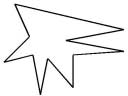
\includegraphics[width=0.7\linewidth]{figs/kiki.png}
  %\caption{Kiki}
  \label{fig:kiki}
\end{subfigure}%
\begin{subfigure}{.5\textwidth}
  \centering
  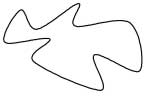
\includegraphics[width=0.7\linewidth]{figs/bouba.png}
  %\caption{Bouba}
  \label{fig:bouba}
\end{subfigure}
  \caption{Demonstration of the ``bouba/kiki effect'' \citep{Ramachandran2001}}
  \label{fig:boubakiki}
\end{figure}

K\"{o}hler found that the vast majority of participants chose to name the sharp, pointy shape `kiki' and the curvy,
rounded shape `bouba'. \citet{Ramachandran2001} found that that this effect holds for 95--98\% of the population. This
is an example of just one audio-visual mapping that is common amongst the population.

%\citep{Hubbard1996}

%These audio-visual associations are not just higher-level constructs that our
%concious brain creates, they affect the brain at the very lowest level even
%with only brief exposure to bimodal stimuli. Zangenehpour et. al.
%\citep{Zangenehpour2010} used a PET-CT scanner to measure blood flow in the
%brain during exposure to audio and visual stimuli. ``When presented with only
%the auditory or visual components of the bimodal stimuli, na\"{i}ve subjects
%showed only modality-specific cortical activation, as expected.  However,
%subjects who had previously been exposed to the audiovisual stimuli showed
%increased cerebral blood flow in the primary visual cortex when presented with
%sounds alone.''

\citet{Spence2011} reviewed a wide range of psychology experiments that attempt to find the inherint cross-modal links
in the human brain, including audio-visual mapping.  There are two common types of test methods used to discover these
links -- `speeded' and `unspeeded'.  In `speeded' tests, participants are tasked with classifying an audio/visual
stimulus and their reaction time is measured. When the auditory and visual stimuli are `congruent' (perceived to be
similar), then their reaction times are quicker. In `unspeeded' tests, visual and audio stimuli are presented very
quickly, one after the other, and participants are asked to select which stimulus came second. When the stimuli are
congruent, participants find it more difficult to work out the order of presentation.
Through his literature review, \citet{Spence2011} found there to be strong evidence for six audio-visual mappings,
which he grouped into three categories, shown in Table~\ref{tab:crossmodal}.

\begin{table}
\centering
\begin{tabular}{|l|l|l|}
\hline
\textbf{Type} & \textbf{Link} & \textbf{Direction} \\ \hline
Structural    & Loudness/brightness  & louder=brighter \\ \hline
\multirow{3}{*}{Statistical} & Pitch/elevation & higher=higher \\ \cline{2-3}
              & Pitch/size & higher=smaller \\ \cline{2-3}
              & Loudness/size & louder=bigger \\ \hline
\multirow{2}{*}{Semantic} & Pitch/elevation & higher=higher \\ \cline{2-3}
              & Pitch/spatial frequency & higher=higher \\ \hline
\end{tabular}
\caption{Audio-visual mappings supported by strong evidence \citep{Spence2011}}
\label{tab:crossmodal}
\end{table}

\citet{Tsiros2014} used a different approach to measure audio-visual crossmodality by using audio visualization
techniques.  Three audio recordings were used -- a violin, recording of wind noise and impact sound event. For each,
images were manually created which used different combinations of audio-visual mappings (e.g. dissonance $\to$ texture
granularity). Participants were played an audio clip and shown an image and were asked whether they are similar or not,
and to what degree (on a scale of 0--100).  The experiment confirmed previous results which found strong links between
size/loudness and pitch/elevation, and weaker links between colour/pitch, granularity/dissonance, and colour
complexity/dissonance.

Additional work from \citet{Marks2003}.

%Vision and audition are physiologically separate, but idential in many respects
%\citep{Tsiros2013}.

In this section, we have seen that the temporal constraints of audio can be overcome by using the spatial properties of
vision. These mappings can be designed to be general, or address specific tasks. There are underlying links between
sound and vision that could be exploited to make more perceptually relevant visualisations.

\subsection{Waveforms}

An audio waveform is the graphical representation of an audio signal. It is perhaps the simplest audio visualisation
technique available and arguably the most commonly used.

% ==== PROS ====

The curve of an audio waveform directly represents the pressure waves of the sound, so the amplitude and frequency of
the sound is mapped to the amplitude and frequency of the plot. This makes it conceptually easy for users to
understand how the audio is represented.

Large curves represent loud sounds, and spatially high frequency curves represent high sound frequencies. These
mappings corrolate with two of the most common cross-modal links (see Table~\ref{tab:crossmodal}).

Waveforms operate in the time domain and can be plotted using a linear function of the audio signal, which makes them
computationally efficient to generate. 

For these reasons, it is the default audio visualisation used in all audio editing software that we have come across.

% ==== CONS ====

In waveforms, frequencies are visible (see Figure~\ref{fig:waveform-zoomin}) at the right scale, but it is hard to work
out which exactly which frequencies are present and in what proportion.

Given a high enough resolution, waveforms can be losslessly be converted back into the original audio signal. In this
sense, they can fully represent the information contained in the audio. However for any practical application, the
time axis of the waveform must be downsampled so that the waveform can be viewed at a reasonable scale (see
Figure~\ref{fig:waveforms}).  This downsampling causes the frequency informaton to be lost, and what remains is the
profile of the audio amplitude.

\citet{Loviscach2011}
proposed an elegant solution to this problem using a technique he calls the `quintessence waveform'. This approach
used extreme pitch shifting to preserve the character of the waveform at different scales (see Figure~\ref{fig:quint}).
Although this approach works well for regular monoaural sounds such as sine waves, it cannot be used for the complex
polyphonic audio used in most real-life applications.

\begin{figure}[p]
\centering
\begin{subfigure}{.5\textwidth}
  \centering
  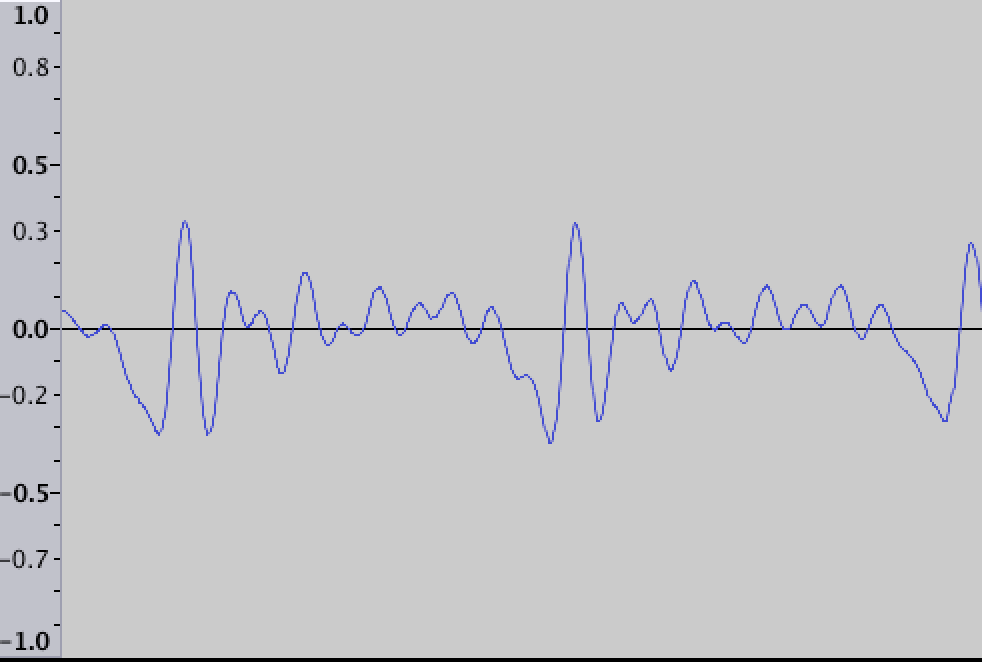
\includegraphics[width=.9\linewidth]{figs/waveform-zoomin.png}
  \caption{When zoomed-in, the frequency information is visible}
  \label{fig:waveform-zoomin}
\end{subfigure}%
\begin{subfigure}{.5\textwidth}
  \centering
  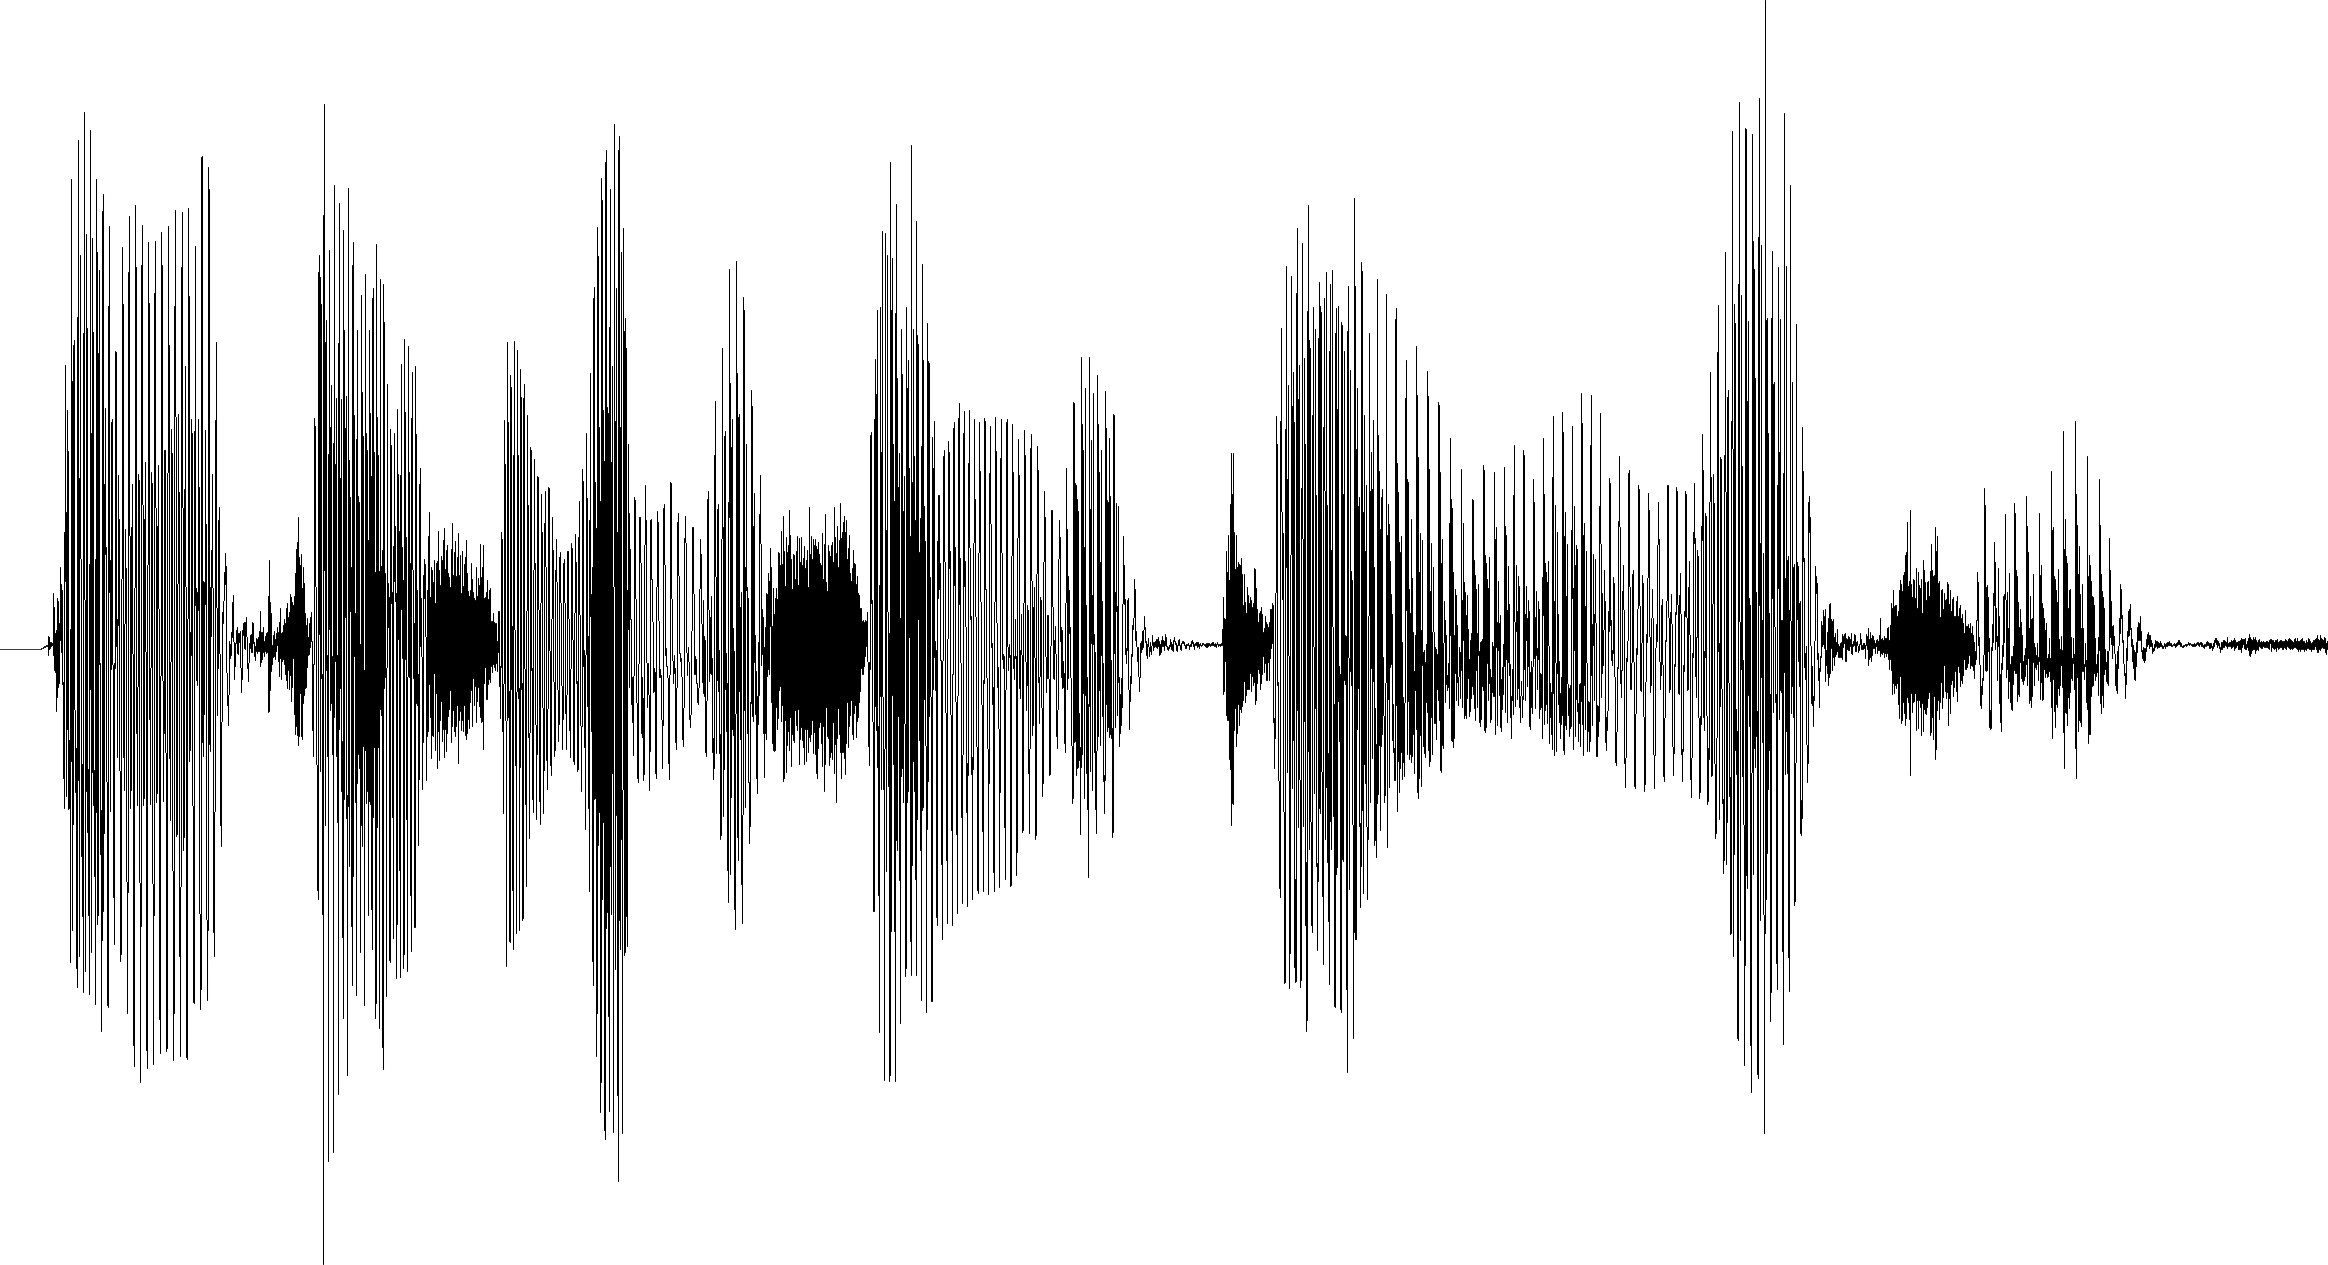
\includegraphics[width=.9\linewidth]{figs/waveform-zoomout.png}
  \caption{When zoomed-out, the frequency information is lost and only the amplitude profile is visible}
  \label{fig:waveform-zoomout}
\end{subfigure}
\caption{The effect of scaling on waveform frequency information}
\label{fig:waveforms}
\end{figure}

\begin{figure}[p]
  \centering
  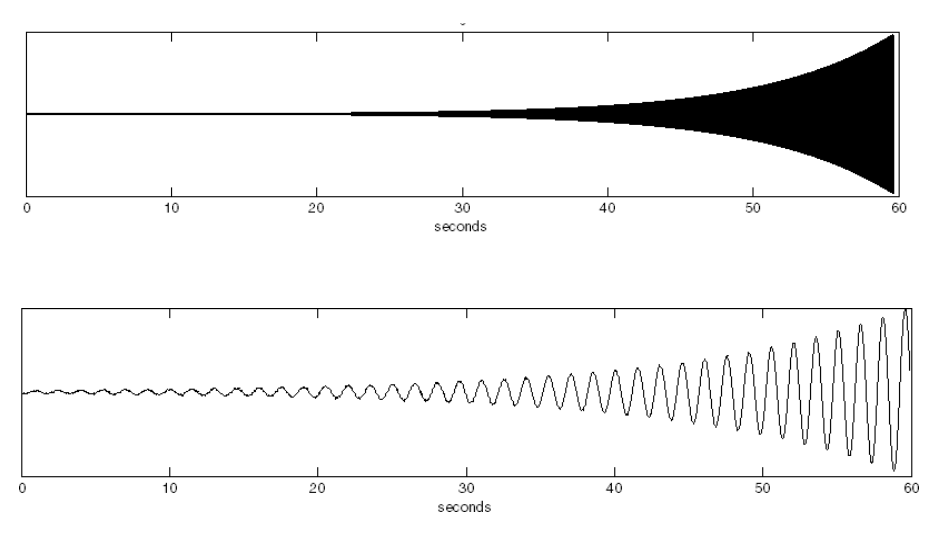
\includegraphics[width=0.95\linewidth]{figs/quint.png}
  \caption{Above: Normal waveform, below: quintessence waveform, source:
  \citep{Loviscach2011}}
  \label{fig:quint}
\end{figure}

\citet{Gohlke2010} proposed a number of ideas for how to improve waveform displays.
%TODO Expand

This amplitude profile can be used to infer some information about the audio content. For example, speech content has
frequent short periods of silence between words, whereas music has few periods of silence. However, in order to be able
to read this information, users must learn what the different profiles of sounds look like.

Many professional engineers and producers have worked with waveforms for most of their career, and have developed the
skills to be able to read waveforms.  However, without frequency content, there is a limit to the amount of information
waveforms can convey.

\subsubsection{User studies}

We searched for studies that considered the performance of waveforms as an interface to audio content. Although X and Y
included waveforms in their studies, the waveforms themselves were not assessed. No studies could be found that
consider the performance of the waveform itself.

\subsection{Spectrograms}
The spectrogram is a visual representation of the spectrum of frequencies in an audio signal over time.  This technique
allows the full frequency content of the audio to be visible to the user. It is a simple mapping that can be easily
understood, and a generic visualisation that can be used for a wide variety of applications.

Unlike waveforms, spectrograms make it easy for the user to see the frequencies that make up the sound, and in what
proportions. When the time axis of spectrograms is rescaled, the frequency information is still visible, so it is much
more robust to scaling than waveforms. This allows a higher density of information at typically-used scales.

The frequency scale in an audio spectrogram is usually presented on a logarithmic or Mel scale to give a better mapping
of frequencies to the perception of pitch. Psuedocolour (see Section~\ref{sec:pseudocolour}) is often used so that the
detail is more visible.

Higher audio frequencies are displayed at the top of the spectrogram, and the energy of the signal is mapped to the
intensity of the colour. Like with waveforms, these corrolate to two of the cross-modal links listed in
Table~\ref{tab:crossmodal}.

Spectrograms are available in most audio editing software, but rarely used by default. As spectrograms are based on a
Fourier analysis, they are more computationally expensive to plot than waveforms, but trivial for modern computers to
generate.

Although spectrograms present the data very clearly, users must still learn how to interpret the information.  
\citet{Zue1986} found that expert users were able to use spectrograms to read the phonemes of speech, but this is
impossible for the average user to achieve.

The spectrogram displays the energy present in each frequency band, however this can make it difficult for the user to
see the overall energy at a given time.

Spectrograms have a wide range of parameters which control how the data is displayed, including window size and 
shape, frequency and energy scaling, min/max values and pseudocolour methods. This means that is a great deal of
inconsistency between spectrogram, which can make it difficult for users to move from one to the other.

Understanding spectrograms requires users to have basic knowledge about how audio is composed of multiple frequencies.
They would also benefit from understanding how frequencies interact, such as harmonics.

%Pros
%X info rich
%X robust to scaling
%X already available
%X simple and generic visualisation
%X computatonally easy

%Cons
%X more computationally expensive than waveforms
%X must learn what different things look like - hard to map frequencies to info
%(doesn't take into account octaves and harmonics)
%X total energy is unclear
%X users must understand that audio is composed of a spectrum of frequencies
%X multiple parameters needed to control visualisation - inconsistent (e.g. window size, window type, 

Spectrograms provide an information-rich and scalable alternative to waveforms, and they are widely available in most
audio editing software. Despite this, waveforms remain a more popular way of interacting with audio. It is unclear as
to why this is.

\subsubsection{User studies}

\citet{Goudeseune2012} used spectrograms as a basis to develop an interface for finding acoustic events.  They filtered
the spectrogram using image processing techniques to create a salience map (see Figure~\ref{fig:timeliner}). This
attempts to dim the background noise to make acoustic events clearer to the user.  Through the use of custom browsing
software called Timeliner, the system was tested by recording how quickly users could find sound effects hidden in long
speech recordings.

\begin{figure}[ht]
  \centering
  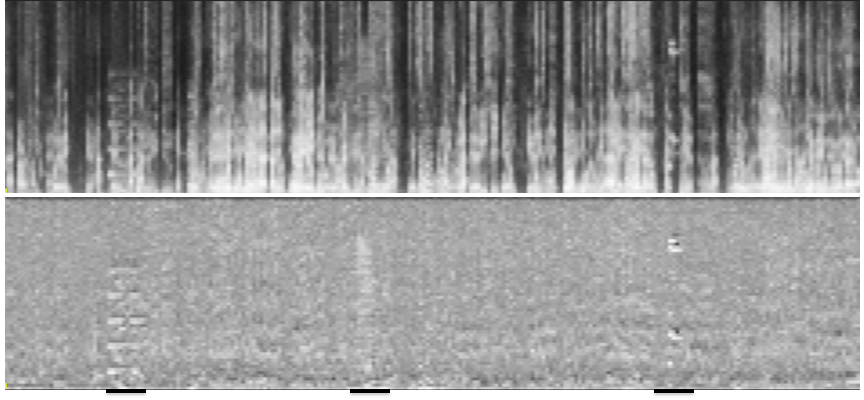
\includegraphics[width=0.95\linewidth]{figs/spectrogram-salience.png}
  \caption{Top: A normal spectrogram; Bottom: A salience-maximised spectrogram with target events marked using black
    underlines}
  \label{fig:timeliner}
\end{figure}

\section{Semantic audio visualisation}\label{sec:semantic}

One of the issues we identified with the above audio visualisations is that the user must interpret the data. Although
in many cases this can be learned, it requires cognitive load to process the images into the desired information. It
also means that novice users must be trained or gain sufficient experience to be able to reach satisfactory performance
levels.

Semantic audio is the extraction of meaning from audio. Example applications of semantic audio are speech-to-text or
music identification. This technology allows the computer to interpret the audio on the user's behalf in a way that is
helpful for their situation, however the success of this is dependent on the performance of the audio analysis
algorithm.

Semantic audio visualisation is a two-stage process where the audio is first analysed to extract the semantic data,
then the data is visualised. There are thousands of audio extraction and data visualisation techniques that could
be combined to create various audio visualisations. The interaction of these two parts, and the context of the
application, is important in the sucess of semantic audio visualisation. 

Below we consider semantic audio visualisation techniques that have attempted to aid navigation of audio content.

%\subsection{Segmentation}
%Music structure
%Speaker diarization

%\subsection{Transcription}
%Music transcription
%Speech to text

\subsection{Colour}\label{sec:colour}
A simple technique that can be used to visualise data is mapping numeric values to colour.  Previous work in the use of
colour for audio visualization can be categorised into two main approaches -- pseudocolour and false colour.

\paragraph{Pseudocolour}\label{sec:pseudocolour}
Pseudocolour is a method of mapping a scalar value to a colour gradient \citep{Moreland2009}.  A tangible example of
pseudocolour is thermal imaging cameras, where temperature is mapped to a colour gradient.  The gradient can be
composed of a two colours (e.g. from blue to red) or many colours (e.g. a rainbow).

Pseudocolour allows values to be mapped to colours that may be more perceptually relevant (e.g. green/red for
good/bad).  It also enables the full colour spectrum to be utilised, which can emphasize small variations between
values.  Non-linear gradients can be used to pick out particularly high or low values, and stepped gradients can be
used to separate values into categories.  However, as pseudocolour can only represent one dimension, it does not make
full use of the colour space.

Spectral waveform colouration has become an increasinly common feature in DJ software. It was first introduced with 
Serato Audio Research's `Scratch LIVE' program.
% TODO What year?
This feature allows DJs to use colour to distinguish between different drum noises, such as bass kicks, snares and
high-hats. Pseudocolour is used to enhanced the waveform, with spectral centroid used as the input audio feature.

The same technique has been applied to other applications, notably on the audio clip sharing website `Freesound' from
Universitat Pompeu Fabra's Music Technology Group\footnote{\url{http://blog.freesound.org/?p=10}, Bram de Jong, Music
  Technology Group, Universitat Pompeu Fabra, Barcelona}. In Freesound, coloured waveforms are used to help users
quickly find and compare sound effect and music clips on the website.

\paragraph{False colour}\label{sec:falsecolour}
False colour is where multiple values are mapped to the dimensions of a colour space. Commonly, three values are
mapped to the RGB (red, green, blue) colour space.  The advantage of this method is that it can make full use of the
available colours.  However, it can be challenging to select three values and map them to colour in a way that humans
can easily understand and interpret.

\citet{Tzanetakis2000} created a visualisation technique known as `Timbregrams' that aimed to ``use color perception
and the pattern recognition capabilities of the human visual system to depict timbral and temporal information''. Their
implementation mapped the first three principal components of a large feature vector to RGB colour space. The authors
claim that this approach matches sounds with similar `textures' to similar colours.
Although the authors didn't combine their algorithm with waveforms, this would be a simple step.

\citet{Rice2005} presented a similar idea to enhance waveforms with colour. The technique is not
explicitly defined, but it maps low/mid/high frequencies to blue/green/red. It was designed for identifying
timbrally distinct sounds and, with training, can be used to identify certain sound effects. Their system has since
been marketed and licensed as `Comparisonics' and has been integrated into commercial audio editing and DJ
software.

\begin{figure}[p]
\centering
\begin{subfigure}{\textwidth}
  \centering
  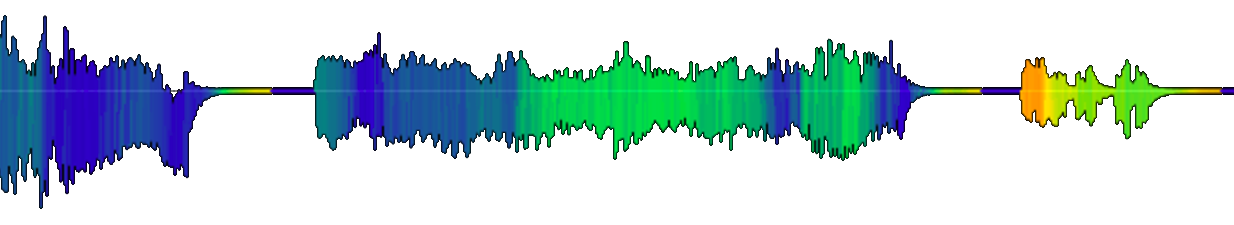
\includegraphics[width=\linewidth]{figs/freesound2.png}
  \caption{Freesound (\url{freesound.com})}
  \label{fig:freesound}
\end{subfigure}\\%
\begin{subfigure}{\textwidth}
  \centering
  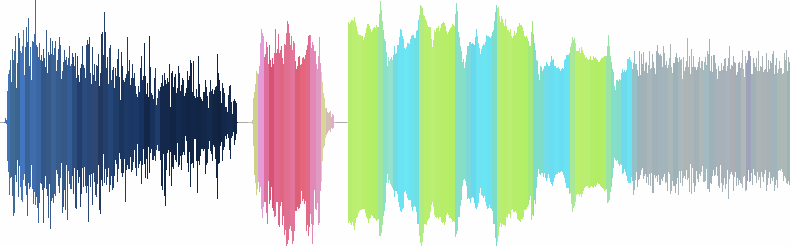
\includegraphics[width=\linewidth]{figs/rice.png}
  \caption{Comparisonics \citep{Rice2005}}
  \label{fig:rice}
\end{subfigure}
\caption{Examples of pseudocolour (\ref{fig:freesound}) and false colour
  (\ref{fig:rice}) applied to colourising an audio waveform}
\label{fig:colourvis}
\end{figure}

\citet{Mason2007} used false colour to assist radio listeners in navigating recently-broadcast material. They mapped
three empirically-chosen audio features to RGB colour space. The authors reported that the system was successful at
indicating the location of music within speech content, and highlighting low-bandwidth material such as phone calls.
The authors proposed that the system could be also be applied to other applications such as segmentation of radio
programmes for re-editing into podcasts.

%Similar work was conducted at the BBC in 2013 by trainee Andrew Bonney who,
%under the supervision of the author, looked into whether colour could represent
%the sound of different people's voices. The result used median-filtered MFCCs
%and gaussian mixture models, mapped to RGB colour space.
%Figure~\ref{fig:bonney} shows an example of a recording with three speakers
%(red/orange, blue and light/dark green).

%\begin{figure}[ht]
  %\centering
  %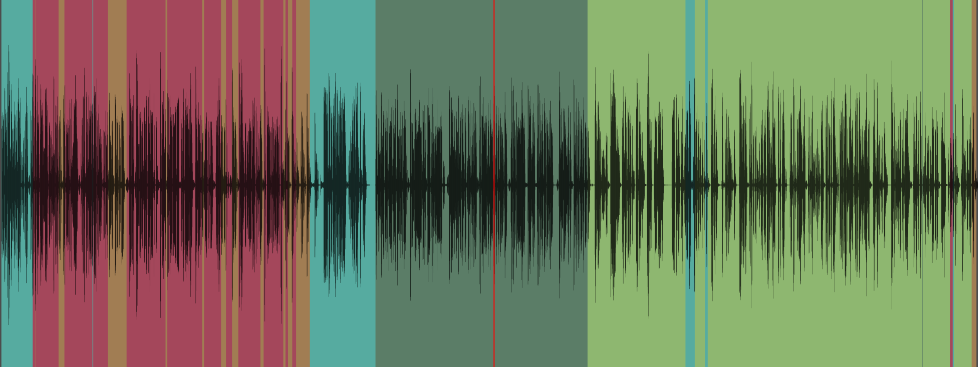
\includegraphics[width=0.95\linewidth]{figs/bonney.png}
  %\caption{Speaker diarizartion through colour based on filtered MFCCs}
  %\label{fig:bonney}
%\end{figure}

False colour has also been used for navigating and summarizing extremely long recordings. \citet{Towsey2014} mapped
three spectral features to RGB colour for visualizing almost a year of environmental recording.
Figure~\ref{fig:towsey} shows the recordings from March until October, with each line representing one day.  The
visualization reveals the change in time of the dawn and evening choruses throughout the year, amongst other things.

\begin{figure}[p]
  \centering
  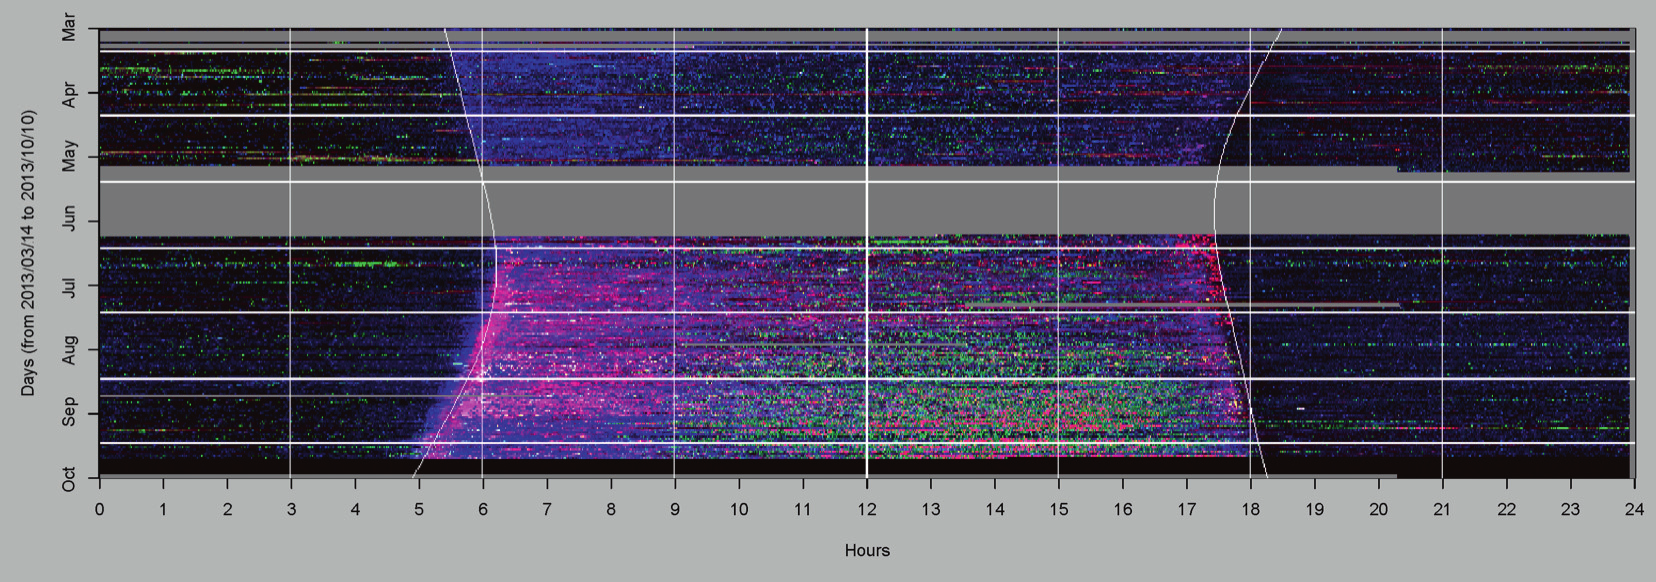
\includegraphics[width=0.95\linewidth]{figs/towsey.png}
  \caption{False colour visualization of environmental recordings, with each line representing one day. Missing data is
    shown in grey.
    \citep{Towsey2014}}
  \label{fig:towsey}
\end{figure}

\subsection{Segmentation}

Speech/music discrimination \citep{Wieser2014}

\subsection{Summarization}

Extracting keyphrases \citep{Inkpen2004}
TreeMaps \citep{Abdulhamid2013a}
World service archive \citep{Raimond2014}

\subsection{Transcripts}

LIDS transcript editor \citep{Apperley2002}

Editor for existing script \citep{Shin2016}


\section{Auditory and haptic interfaces}\label{sec:auditory}

SpeechSkimmer \citep{Arons1997}

Dichromatic listening \citep{Ranjan2006}

Haptics
\citep{Metatla2016}

%======================================================================================================================

%Academic research into audio analysis and audio interfaces tends to concentrate
%on fully automated systems \citep{AngueraMiro2012}, navigation of large audio
%collections \citep{FontCorbera2010} or navigation interfaces based on skimming
%\citep{Arons1997} and scrolling \citep{Lee2007}. Although there are examples of
%audio visualization from the world of academia, it is much more popular in the
%context of art \citep{Armitage2012}, with excellent examples such as Quayola's
%Form--Sound--Abstraction\footnote{\url{http://www.quayola.com/work/form-sound-abstraction/}}
%work.

%This section looks at three areas of literature from which the project will
%draw upon -- extraction of meaningful audio properties, mapping these to a
%visual representation, and the perceptual links between audition and vision.

%\section{Feature extraction}\label{sec:litreviewfeats}
%This section looks at audio features that could be used as part of an audio
%visualization system. Firstly, two use cases that were previously identified as
%being a common component of radio production are explored, before considering
%methods of generating features for any use case.

%\subsection{Speech/music discrimination}
%Speech/music discrimination (SMD) is the process of segmenting audio content
%into parts labelled by the categories speech and music. In general, SMD
%classifiers use a collection of different features. This section lists the ones
%that are used frequently or have recently been found to perform well.

%\paragraph{RMS energy}
%The root mean squared energy can be used also exclusively as an effective SMD
%classifier, as demonstrated in \citep{Ericsson2009} and \citep{Panagiotakis2005}.
%Commonly used statistics of RMS include low energy ratio
%\citep{Liang2005,Ericsson2009,Saunders1996,Scheirer1997} and variance
%\citep{Ericsson2009} (including normalised variance \citep{Panagiotakis2005} and
%delta variance \citep{Carey1999}).

%Low energy ratio (also known as `silent interval frequency' and `energy contour
%dip') is a measure of the number of RMS energy frames that fall below a
%threshold. It exploits the fact that speech has freqent silent gaps between
%words, wheras music does not. The threshold can be set as a fixed value
%\citep{Liang2005}, a function of a moving average \citep{Ericsson2009} or moving
%peak value \citep{Saunders1996}.

%Kacprzak and Zi\'{o}\l{}ko recently proposed a modified version of low energy
%ratio called `minimum energy density' \citep{Kacprzak2013}. It is calculated by
%normalizing over a $\sim$15 second window and finding the minimum of the
%normalization function over a $\sim$1--3 second window. It has similar
%performance to low energy ratio with a moving average threshold, but has fewer
%parameters to set.

%\paragraph{Zero-crossing rate} is the rate at which a signal crosses the time
%axis, which is an easy-to-calculate measure for the spectral energy
%distribution. Early work in SMD \citep{Saunders1996} identified that ``speech
%signals produce a marked rise in the ZCR during periods of fricativity occuring
%at the beginning and end of words'', wheras music does not. This causes a
%bimodality which skews the ZCR distribition, which can be measured using the
%third standardized moment (skewness). The variance of ZCR has also been found
%to perform well for SMD \citep{Scheirer1997}.

%ZCR also played a significant role in two steps of a five-step classifer
%\citep{Panagiotakis2005}. During silent intervals the number of zero crossings
%is null, so this was used to detect gaps between speech. The authors also noted
%that ``RMS and ZCR are somewhat correlated for speech signals, while
%essentially independent for music'', and so the product of RMS and ZCR was used
%for the second classifier.

%A review \citep{Carey1999} of features for SMD found ZCR to perform least well,
%but did not consider the skewness, variance, or probability of null
%zero-crossings.

%\paragraph{MFCC}
%Mel-frequency cepstral coefficients have long been the workhorse of audio
%analysis, and they have been successfully used in SMD applications
%\citep{Carey1999,Liang2005,Pikrakis2008,Pikrakis2006a,Sell2014,Wieser2014}.
%Notably, their use has only been successful when used in combination with
%strong machine learning systems, indicating that the relationship of MFCCs to
%SMD labels is complex and non-linear. This would make it difficult to map to a
%visual representation.

%\paragraph{Chroma}
%Use of chroma features work on the principle that the spectra of music is
%aligned to the chromatic scale. Pikrakis et. al.
%\citep{Pikrakis2006,Pikrakis2008} have successfully used `chromatic entropy' for
%SMD applications. It takes sub-bands from a mel-scaled spectrum, aligned to the
%chromatic scale, and calculates the entropy of the normalised spectral energy.

%More recently, Sell \citep{Sell2014} has proposed two new chroma features, which
%try to account for the fact that the chromagram varies greatly between
%different pieces of music. Music tends to form strong, separated peaks on the
%chromagram wheras speech has smoother mounds of energy. The new features
%attempt to measure the peakiness of the chromagram. `Chromatic diff' subtracts
%a shifted chroma vector from the original chroma vector and sums the energy. 
%`Chroma high freq' performs an FFT on the chromagram and sums the high
%frequency energy.

%\paragraph{Continuous frequency activation}
%Most of the above SMD features work well for segmenting speech-only/music-only
%content. However, many fall down at detecting background music in speech.
%Seyerlehner developed the continuous frequency activation (CFA) feature
%\citep{Seyerlehner2007}, which works on the basis that music content has stable
%harmonics, seen as horizontal lines on a spectrogram.

%A moving average is subtracted from the FFT before it is binarized using a low
%threshold value. For each bin, the proportion of active frames in an analysis
%window is counted. The result is analysed with a peak picking algorithm and the
%sum of the five largest peaks are used as the CFA. The result is a single
%numeric value which quantifies the presence of steady frequency components.

%In the original CFA paper, the feature was used to find music in television
%content, but recently it has also been successfully applied to segmentaton of
%radio recordings \citep{Wieser2014}.

%\subsection{Speaker diarization}
%Speaker diarization is the process of segmenting a speech recording by where
%different people are talking. Review papers from 2006 \citep{Tranter2006} and
%2012 \citep{AngueraMiro2012} show that the vast majority of systems are based on
%clustering of MFCC or PLP features, which are low-dimensional representations
%of speech. Rather than developing new features, the research is primarily
%focussed on improvement of the clustering algorithms and pre-processing stages
%such as Wiener filtering, speech activity detection and beamforming.

%MFCC and PLP features are extremely effective when used in machine-based
%classification systems, but from a human perception angle, the features do not
%correlate well to what is heard.  Other features developed for automatic speech
%recognition may also be useful in a speaker diarization system. For example,
%spectral entropy \citep{Misra2004} is a measure of the peakiness of the spectrum
%and is an effective feature in distinguishing between voiced and unvoiced
%speech.

%Friendland et. al. \citep{Friedland2009} proposed enhancing the standard MFCC
%features with a set of long-term features representing prosody (the rhythm and
%intonation of speech). 52 candidate features were ranked using feature
%selection, which showed that ``the median and mean fundamental frequency are
%the best features, following by high formants (F4, F5)''. Inclusion of the
%top ten prosodic features improved the speaker diarization system by 24\%.

%\subsection{Feature generation}\label{sec:litreviewgeneration}
%Traditionally, audio features were developed by hand for specific tasks. This
%was usually done by attempting to write an algorithm that calculated the
%properties of the sound that humans used to distinuish the categories in
%question. More recently, fuelled by an ever-increasing availability of
%computing power, research has had a much greater focus on automating
%this process.

%\paragraph{Feature selection/extraction}
%Feature selection and extraction are methods of reducing the dimensionality of
%a feature vector, either by choosing a combination of vector components that
%best describe the content (selection), or by translating the feature vector to
%a smaller vector while retaining as much information as possible (extraction).

%This process can be unsupervised where only the feature data is known (such as
%with principal component analysis), or supervised where the feature data has
%corresponding labels (such as with linear discriminant analysis).

%Canonical correaltion analysis (CCA) has been used to reduce the dimensions of
%features for speaker diarization \citep{Chaudhuri2009} and phonetic labelling
%\citep{Arora2014}, amongst other things. It is able to efficiently map features
%to a subspace and can be used with the kernel trick (known as KCCA) to support
%non-linear mappings. In the case of speaker clustering, ``CCA-based algorithms
%consistently provide better performance than standard PCA-based clustering
%methods'' \citep{Chaudhuri2009}.

%\paragraph{Feature learning}
%The above methods of reducing dimensionality are based on a relatively short
%information-rich feature vector that it suitable for the target application.
%More recent research on feature development is focussed on automated learning
%of features using large labelled datasets.

%Deep learning is an increasingly popular method of learning features based on
%neural networks with large numbers (tens or hundreds) of hidden units. This
%line of research has been enabled by the increasing availability of large
%amount of processing power. When done properly, deep learning can produce the
%state-of-the-art in audio features, outperforming even the best hand-crafted
%features \citep{Hamel2010,Sigtia2014}.

%Such an approach requires a high-quality and very large labelled dataset, on
%which the success of the process depends. The nature of neural networks means
%that it is very difficult to interpret what the resulting features represent
%which isn't an issue when used as the input to a machine learning system, but
%would make it very difficult to map to a visualization. The objective of the
%deep learning process is to minimise a cost function rather than to maximise
%the link to human perception.
